
\chapter[Related Works]{State of the art}
\graphicspath{ {images/stateOfArt} }



\section{Software visualization}


\begin{wrapfigure}{r}{0.3\textwidth}

  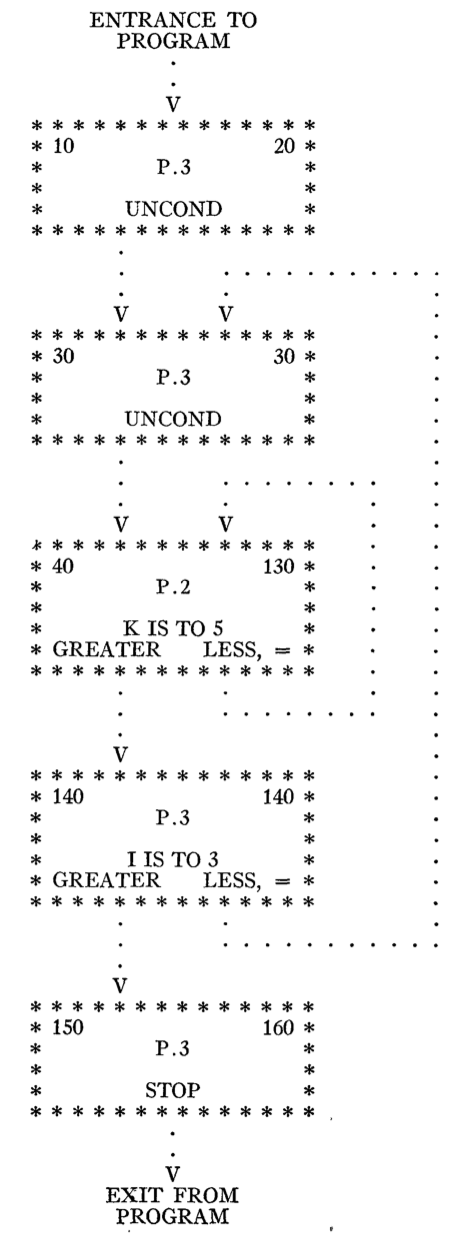
\includegraphics[width=0.9\linewidth]{Haibt1959_Flowchart.png} 
  \caption{Flowchart presented by Haibt in 1959}
  \label{fig:Haibt1959_Flowchart}

\end{wrapfigure}

Software maintenance and evolution are essential parts of the software development lifecycle. Both require that developers deeply understand their system. 
Mayrhauser and Vans defined {\it program comprehension} as a process that "{\it knowledge to acquire new knowledge}" \cite{VonMayrhauser1995}. 
Generally, programmers possess two types of knowledge: general knowledge and software-specific knowledge. 
Software comprehension aims to increase this specific knowledge of the system, and it can leverage some software visualization techniques for this purpose. 
Software visualization supports the understanding of software systems
by visually presenting various information about them, e.g., their architecture, source code, or behavior.
Stasko et al.\cite{Stasko2008} conducted a study in 1998 that shows how visualization arguments human memory since 
it works as external cognitive aid and thus, improves thinking and analysis capabilities.

\bigbreak

There are cases when software visualization can be used to aid the analysis activity. For example, when programmers need to comprehend the architecture of a system \cite{Panas2007}, when researchers analyze version control repositories \cite{Greene2017}, or to support developers' activity \cite{LopezHerrejon2018}. \\
\\
According to Butler et. al. \cite{Butler1993} there are three categories of visualization:
\begin{itemize}
	 \item Descriptive visualization. Widely used for education purposes, the visualization is used to present data to other people. 
	 \item Explorative visualziation. Used to discover the nature of the data being analyzed. With this visualization, the user usually does not know what he/she is looking for. 
	 \item Analytical visualization. Adapted when we need to find something known in the available data. 
\end{itemize}
	Dijkstra1971a
All the software visualization approaches vary with respect to two dimensions: the level of abstraction and the visualized data.
According to the type of the data, we can classify visualization as:
\begin{itemize}
	\item Evolutionary visualizations. Used to present information extracted from the history of a system. Mainly used to find the cause of problems in software. 
	\item Static visualizations. Used to present information extracted with static analysis of the software. It provides information about the structure of the system.
	\item Dynamic visualizations. Used to present information extracted with dynamic instrumentation of the software execution. It provides information about the behavior of the system.
\end{itemize}

Moreover, the level of abstraction can be classified as:
\begin{itemize}
	\item Code-level visualization. Used to visualize fine granted sourcecode information, such as the lines of code. 
	\item Design-level visualization. Used to visualize self-contained pieces of code, such as classes in object-oriented systems. 
	\item Architectural-level visualization. Used to visualize the system architecture and the relationships among its components. 
\end{itemize}


% \subsection*{History of software visualization}


\bigbreak

The earliest software visualization techniques in the literature used 2D diagrams. 
For example, Haibt, the first to use them in 1959, provided a graphical outline of a program and its behavior with flowcharts \cite{Haibt1959}. 
As shown in Figure \ref{fig:Haibt1959_Flowchart}, they were 2D diagrams that described the execution of a program.
He wrapped each statement in a box, representing the control flow with arrows.

 \bigbreak
Ten years later, Knuth also confirmed the effectiveness of flowcharts \cite{Knuth1963}. 
He evidenced that programs around that time were affected by a lack of readability.
Therefore, he introduced a tool to generate visualizations from the software documentation automatically.

\bigbreak
Nassi and Schneiderman\cite{Nassi1973}, in 1973, introduced the Nassi–Shneiderman diagram (NSD), able to represent the structure of a program. 
The diagram was divided into multiple sub-block, each with a given semantic based on its shape and position. 

\bigbreak
The 80s registered two main directions of software visualization. The first was the source code presentation.
For example, Hueras and Ledgard \cite{Hueras1977} then Waters \cite{Waters1983} developed techniques to format the source code with a prettyprinter. 
The second direction was the program behavior, used mainly for educational purposes.
 
\bigbreak
One of that period's most prominent visualization systems was Balsa-II \cite{Brown1988}.
Balsa-II was a visualization system that, through animations, displayed the execution of an algorithm.
Programmers were able to customize the view and the control execution of the algorithm, to understand them with a modest amount of effort. 
The program was domain-independent, and learners could use it with any algorithm. 

\bigbreak
Around the end of the 80s, Müller et al. \cite{Mueller1988} released Rigi, a tool used to visualize large programs.
It exploited the graph model, augmented with abstraction mechanisms, to represent systems components and relationships. 

\begin{figure}[H]
  \minipage{0.33\textwidth}
    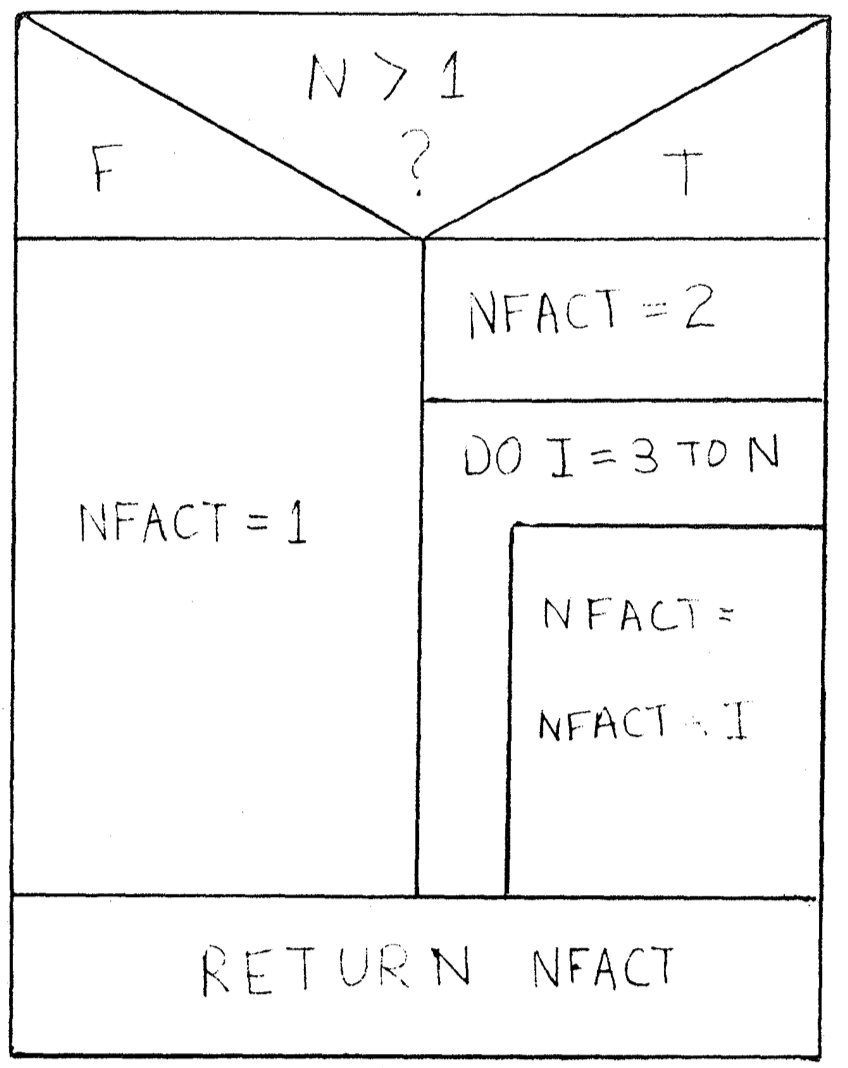
\includegraphics[width=0.8\linewidth]{Nassi1973_NSD.png}
    \label{fig:Nassi1973_NSD}
    \caption{NSD of the factorial function.}
  \endminipage\hfill
  \minipage{0.33\textwidth}
    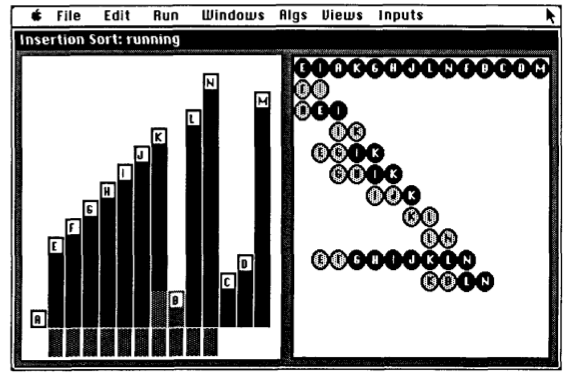
\includegraphics[width=\linewidth]{Brown1988_BalsaII.png}
    \caption{Balsa-II}
  \endminipage\hfill
  \minipage{0.33\textwidth}
  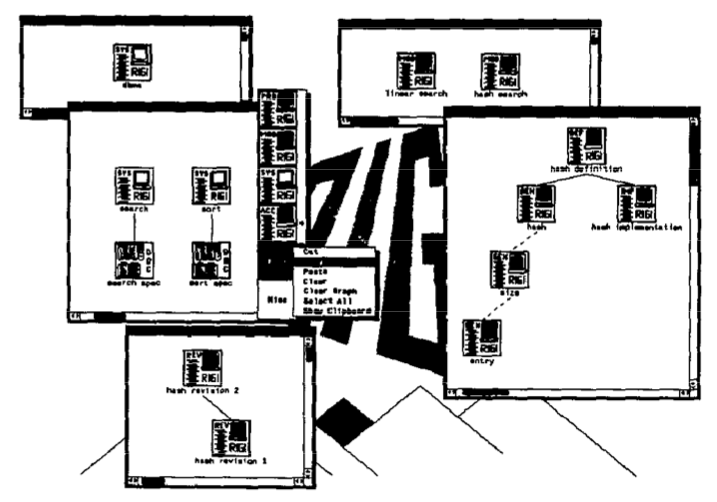
\includegraphics[width=\linewidth]{Mueller1988_Rigi.png}
  \caption{Rigi}
\endminipage\hfill
  \end{figure}


  % The growing number of object-oriented programming languages emerging in the mainstream raised 
  % the interest in understanding not only the structure but also the behavior of systems written according to this paradigm. 
  % Kleyn et al. proposed GraphTrace [KG88], a tool using concurrently animated views to visualize dynamic information,
  % Myers's taxonomy of program visualization systems
  % Price et al. proposed a more detailed taxonomy

\bigbreak
The 1990s recorded more interest in the field of software visualization. 
In 1992, Erik et al. introduced a new technique to visualize line-oriented statistics \cite{Eick1992}. 
It was embodied in Seesoft, a software visualization system to analyze and visualize up to 50,000 lines of code simultaneously. 
On their visualization, each line was mapped to a thin row. Each row was associated with a color that described a statistic of interest.

\bigbreak
One year later, De Pauw et al. \cite{DePauw1993} introduced Jinsight, a tool able to provide animated views of object-oriented systems' behavior. 

\begin{figure}[H]
  \minipage{0.5\textwidth}
    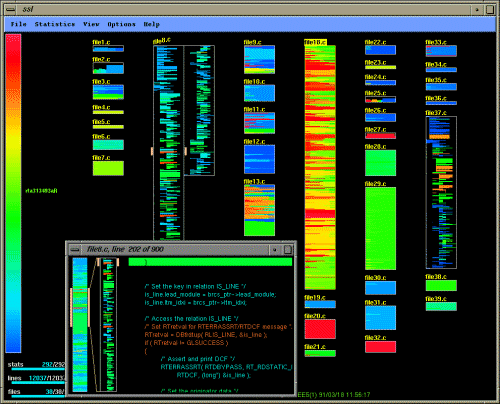
\includegraphics[width=0.8\linewidth]{Eick1992_Seesoft.png}
    \caption{Seesoft}
  \endminipage\hfill
  \minipage{0.5\textwidth}
    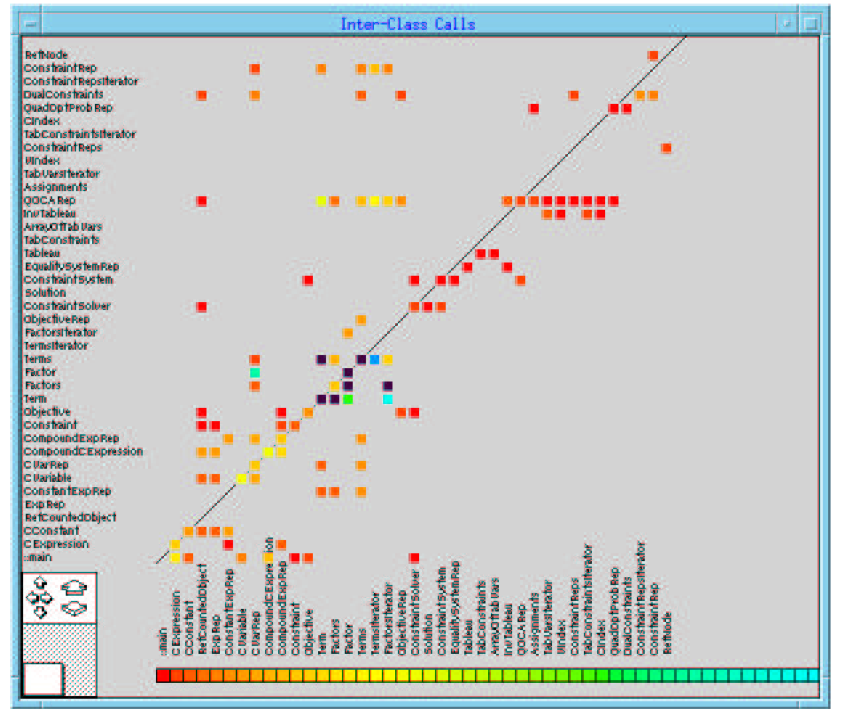
\includegraphics[width=0.8\linewidth]{DePauw1993_Jinsight.png}
    \caption{Jinsight}
  \endminipage\hfill
\end{figure}

% the first contributors to software evolution visualization were Holt and Pak in 1996, who used their tool called GASE [HP96]
% 		GASE: visualizing software evolution-in-the-large 

That period was favorable also for experimenting with novel research directions for visualization, 
such as 3D visualization and Virtual Reality. 


% In 1995, Reiss presented a configurable engine for building 3D visualization of programs called PLUM
\bigbreak
In 1998, Chuah and Erick \cite{Chuah1998} proposed three different techniques to visualize project data. 
They exploited the concept of glyphs, a graphical object that represents data through visual parameters. 
The first technique was the Timewhell glyph, used to visualize time-oriented information (number of lines of code, number of errors, number of added lines). 
The second technique was the 3D wheel glyph; it encoded the same attributes of the time wheel, and additionally, it used the height to encode time. 
Infobug glyph was the last technique, where each glyph was composed of four parts, each representing essential data of the system, such as time, code size, and the number of added, deleted, or modified code lines. \newline

\begin{figure}[H]
\minipage{0.32\textwidth}
  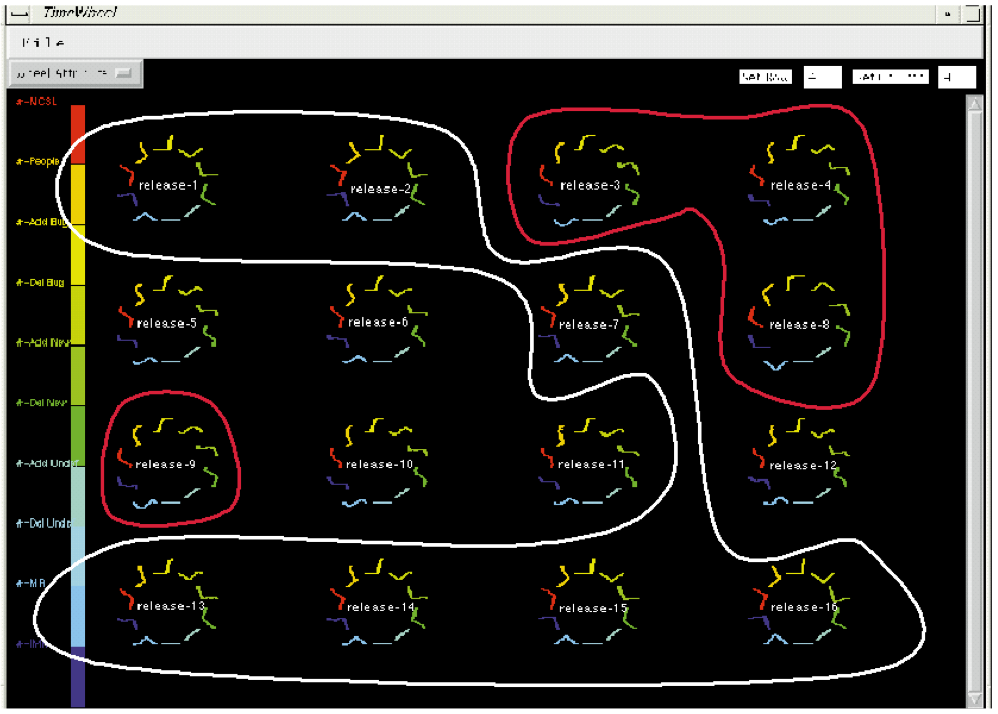
\includegraphics[width=\linewidth]{Chuan1.png}
  \caption{Timewhell}
\endminipage\hfill
\minipage{0.32\textwidth}
  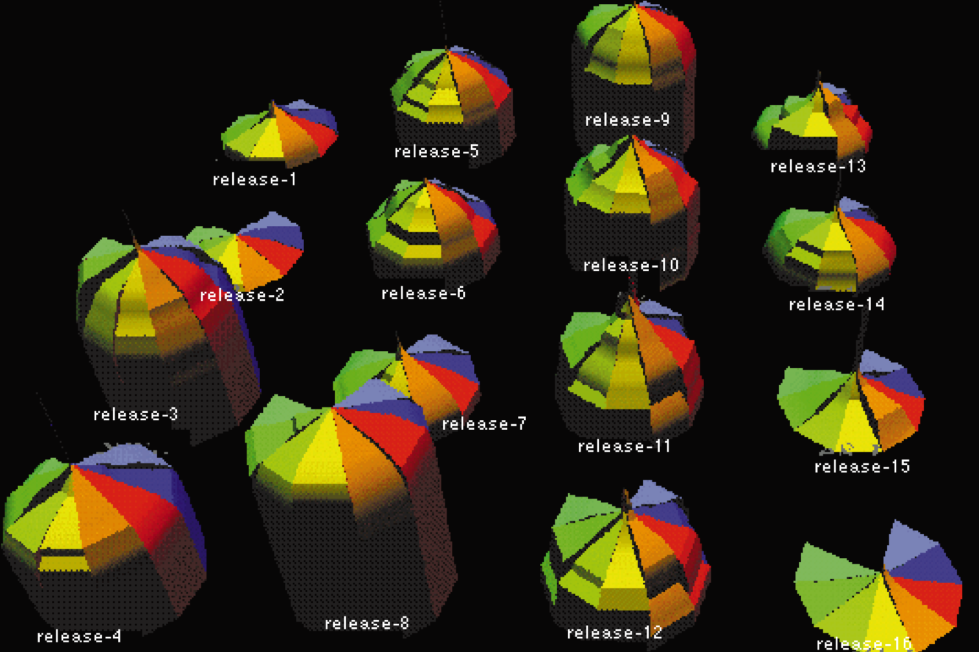
\includegraphics[width=\linewidth]{Chuan2.png}
  \caption{3D wheel}
\endminipage\hfill
\minipage{0.32\textwidth}%
  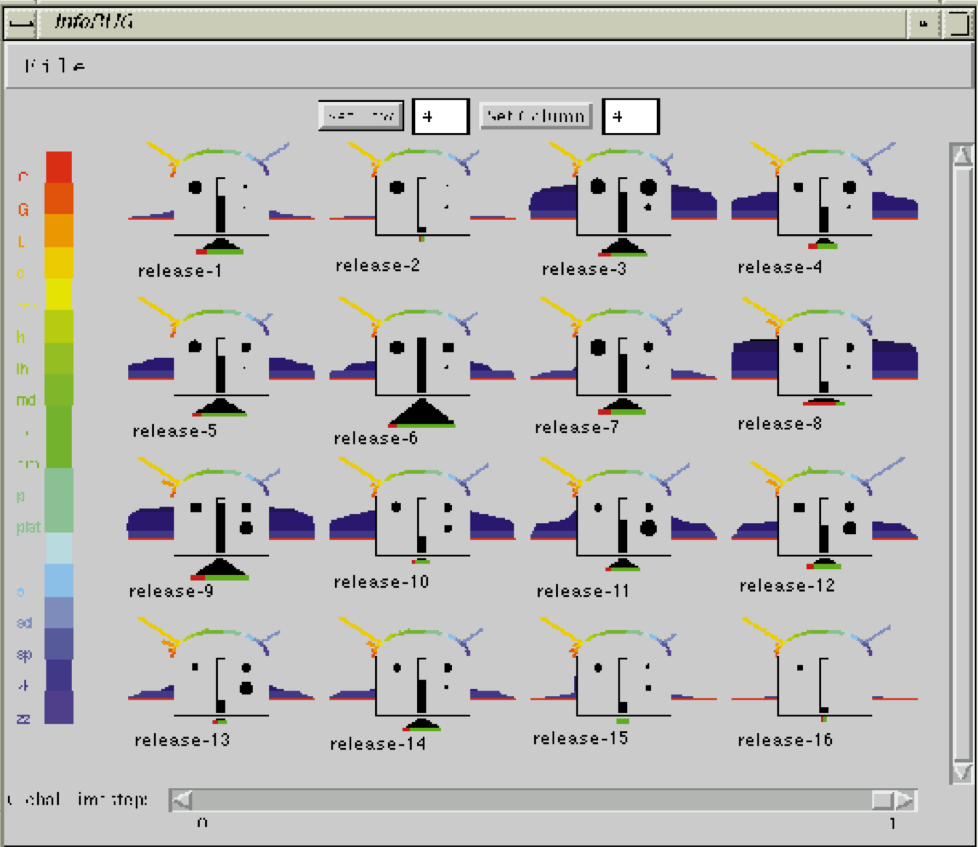
\includegraphics[width=\linewidth]{Chuan3.png}
  \caption{Infobug}
\endminipage
\end{figure}
 
\bigbreak
Also in 1998, Young and Munro \cite{Young1998} explored representations of software for program comprehension in VR. 

\bigbreak
Finally, in 1999, Jacobson et al. \cite{Jacobson1999} introduced what we now know as de facto the standard language to visualize the design of a system: UML. 


% Edward Tufte has influenced the entire field of information visualization, including software visualization.
% 	[Tuf90] Edward Tufte. Envisioning Information. Graphics Press, 1990.
% 	[Tuf97] Edward Tufte. Visual Explanations. Graphics Press, 1997.
% 	[Tuf01] Edward Tufte. The Visual Display of Quantitative Information. Graphics Press, 2nd edition, 2001.

% \subsection{Software evolution visualization}
%https://www.inf.usi.ch/faculty/lanza/Downloads/Gall2006a.pdf
\bigbreak
At the beginning of the 21st century, thanks to the spread of version control systems and the open-source movement, 
visualizing a software system's evolution became a more feasible activity thanks to publicly accessible system information.   
As a result, many researchers focused their work on software evolution visualization.

\bigbreak
Lanza \cite{Lanza2001} introduced the concept of the Evolution Matrix. 
It was a way to visualize the evolution of software without dealing with a large amount of complex data. 
Furthermore, this approach was agnostic to any particular programming language. 
The Evolution Matrix aimed to display the evolution of classes in object-oriented software systems. 
Each column represented a version of the software; each row represented a different version of the same class.
Cells were filled with boxes whose size depended on evolutionary measurements. 
The shape of the matrix could also be used to infer various evolutionary patterns.

\begin{figure}[H]
\minipage{0.49\textwidth}
  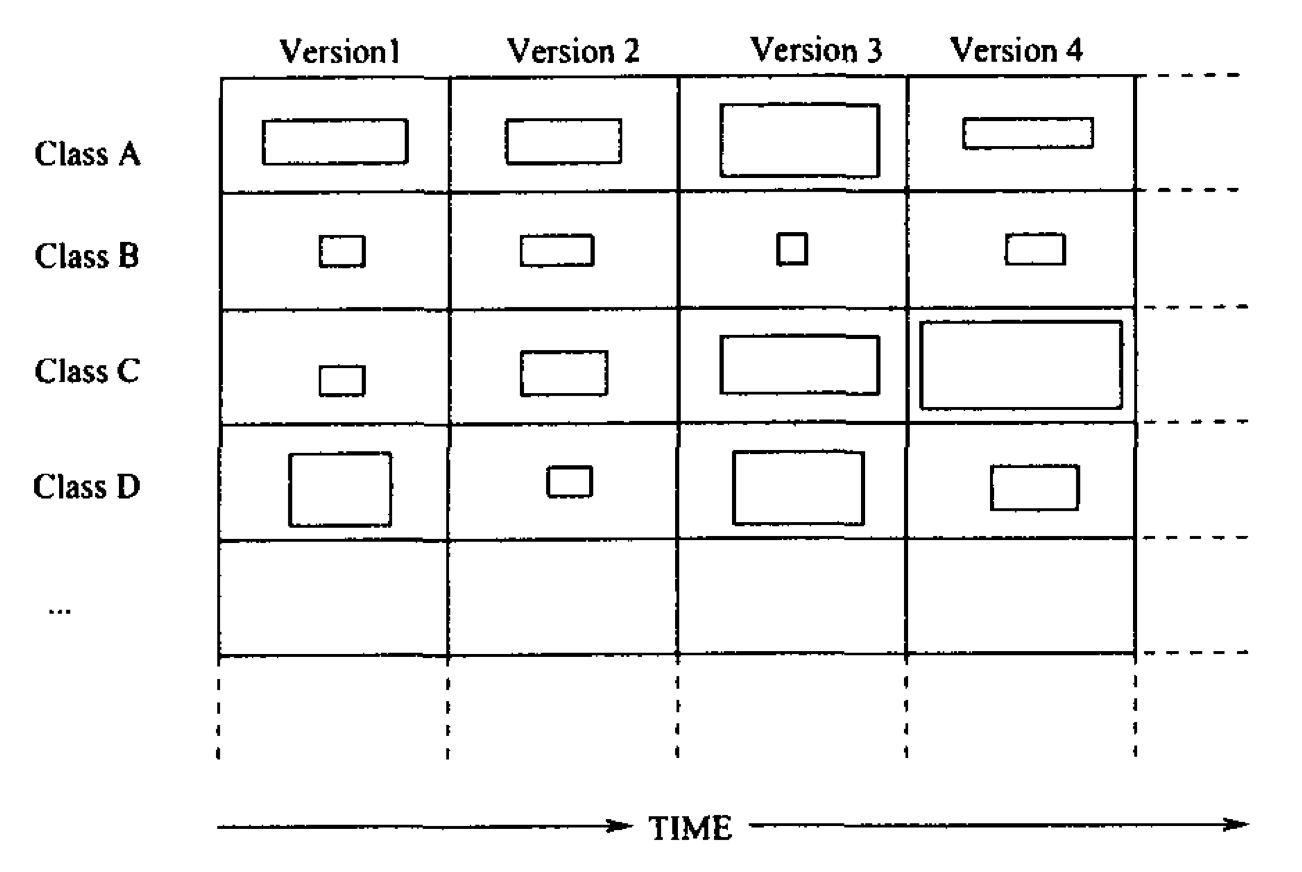
\includegraphics[width=\linewidth]{EvolutionMatrix1.png}
  \caption{A schematic display of the Evolution Matrix}
\endminipage\hfill
\minipage{0.49\textwidth}
  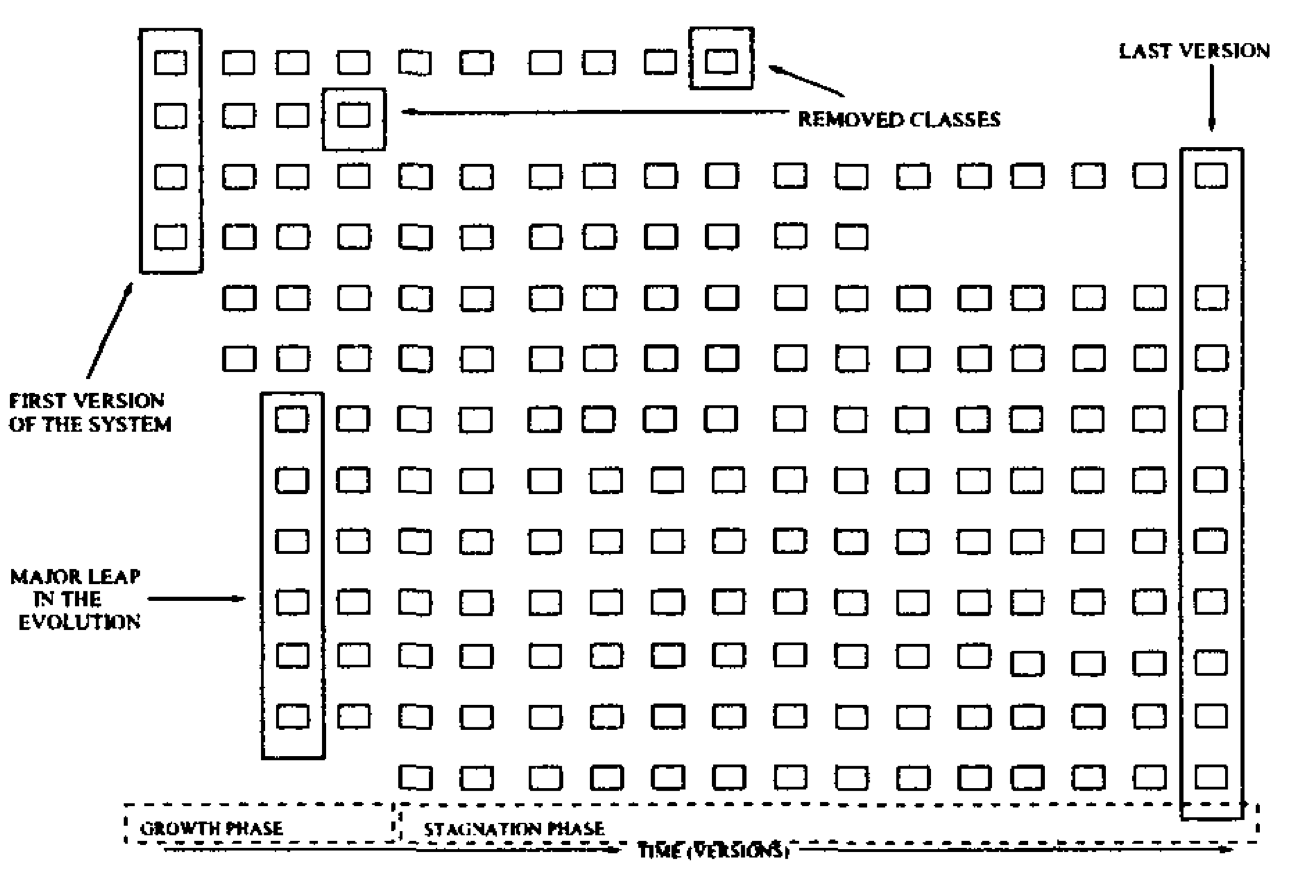
\includegraphics[width=\linewidth]{EvolutionMatrix2.png}
  \caption{Some characteristics of the Evolution Matrix}
\endminipage\hfill
\end{figure}

\bigbreak
Taylor and Munro \cite{Taylor2002},  demonstrated that it was possible to use the data contained in a version control repository to visualize the evolution of a system.
They developed Revision Tower, a tool that showed change information at the file level. 
Pinzger et al. \cite{Pinzger2005} visualized the evolution of a software system through Kivat diagrams.
RelVis, their tool, was able to depict a multivariate visualization of the evolution of a system.

\bigbreak
During the same year, Ratzinger et al. presented EvoLens \cite{Ratzinger2005}, a visualization approach and tool to 
explore evolutionary data through structural and temporal views.

\bigbreak
Langelier et al. \cite{Langelier2005} investigated the interpretation of a city metaphor 
\cite{Knight2000} to add a new level of knowledge to the visual analysis.
 
\bigbreak
D’Ambros and Lanza \cite{DAmbros2006} introduced the concept of Discrete-Time Figure concept. It was a visualization technique that embedded historical and structural data in a simple figure. 
Their approach depicted relationships between the histories of a system and bugs. 
They also presented the Evolution Radar \cite{DAmbros2006a}, a novel approach to visualize module-level and file-level logical coupling information.

\begin{figure}[H]
  \minipage{0.33\textwidth}
    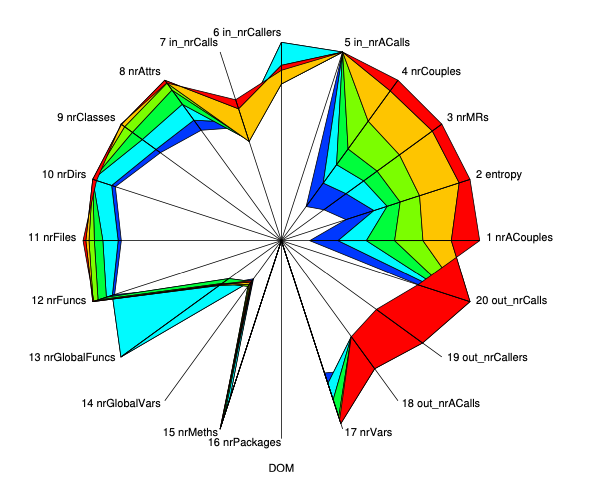
\includegraphics[width=\linewidth]{Pinzger2005_RelVis.png}
    \caption{RelVis}
  \endminipage\hfill
  \minipage{0.33\textwidth}
    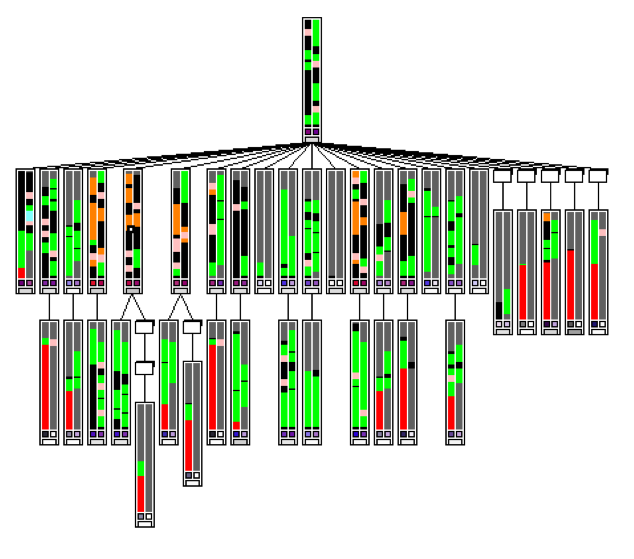
\includegraphics[width=\linewidth]{DAmbros2006.png}
    \caption{Tree of Discrete Time Figures}
  \endminipage\hfill
  \minipage{0.33\textwidth}
  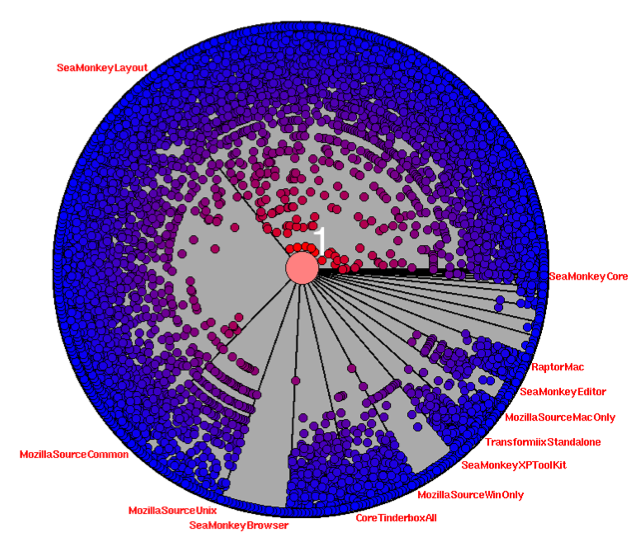
\includegraphics[width=\linewidth]{DAmbros2006a_EvoRadar.png}
  \caption{Evolution Radar}
\endminipage\hfill
  \end{figure}
  
  \bigbreak
Steinbrückner and Lewerentz \cite{Steinbrueckner2010} described a three-staged visualization approach to visualize large software systems. 
Thir visualization was supported by a tool called Evo-Streets. 
Each stage of their approach was responsible for representing a different aspect of the system with the city metaphor. 


\begin{figure}[H]
  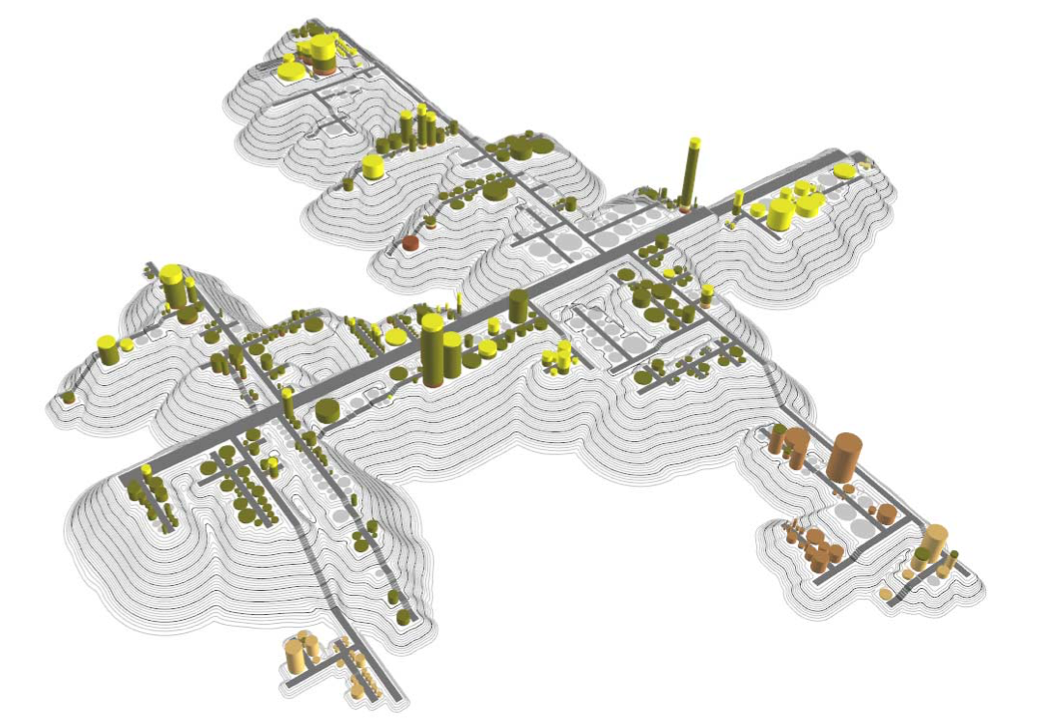
\includegraphics[width=0.9\linewidth]{Steinbrueckner2010.png} 
  \caption{Evo-Streets}
\end{figure}
 
\bigbreak
Wettel revised the city metaphor to represent metrics meaningfully  \cite{Wettel2011}. 
In his thesis, he represented packages as districts and classes as buildings.
The metaphor was used for various purposes, e.g., reverse engineering, program comprehension, software evolution, or software quality analysis. 
He claimed that the city metaphor brought visual and layout limitations; for example, not all visualization techniques fit well.
Under those circumstances, he preferred simplicity over the accuracy,
so he obtained a simple visual language that facilitated data comprehension. His approach was implemented as a software visualization tool 
called CodeCity. 


\begin{figure}[H]
  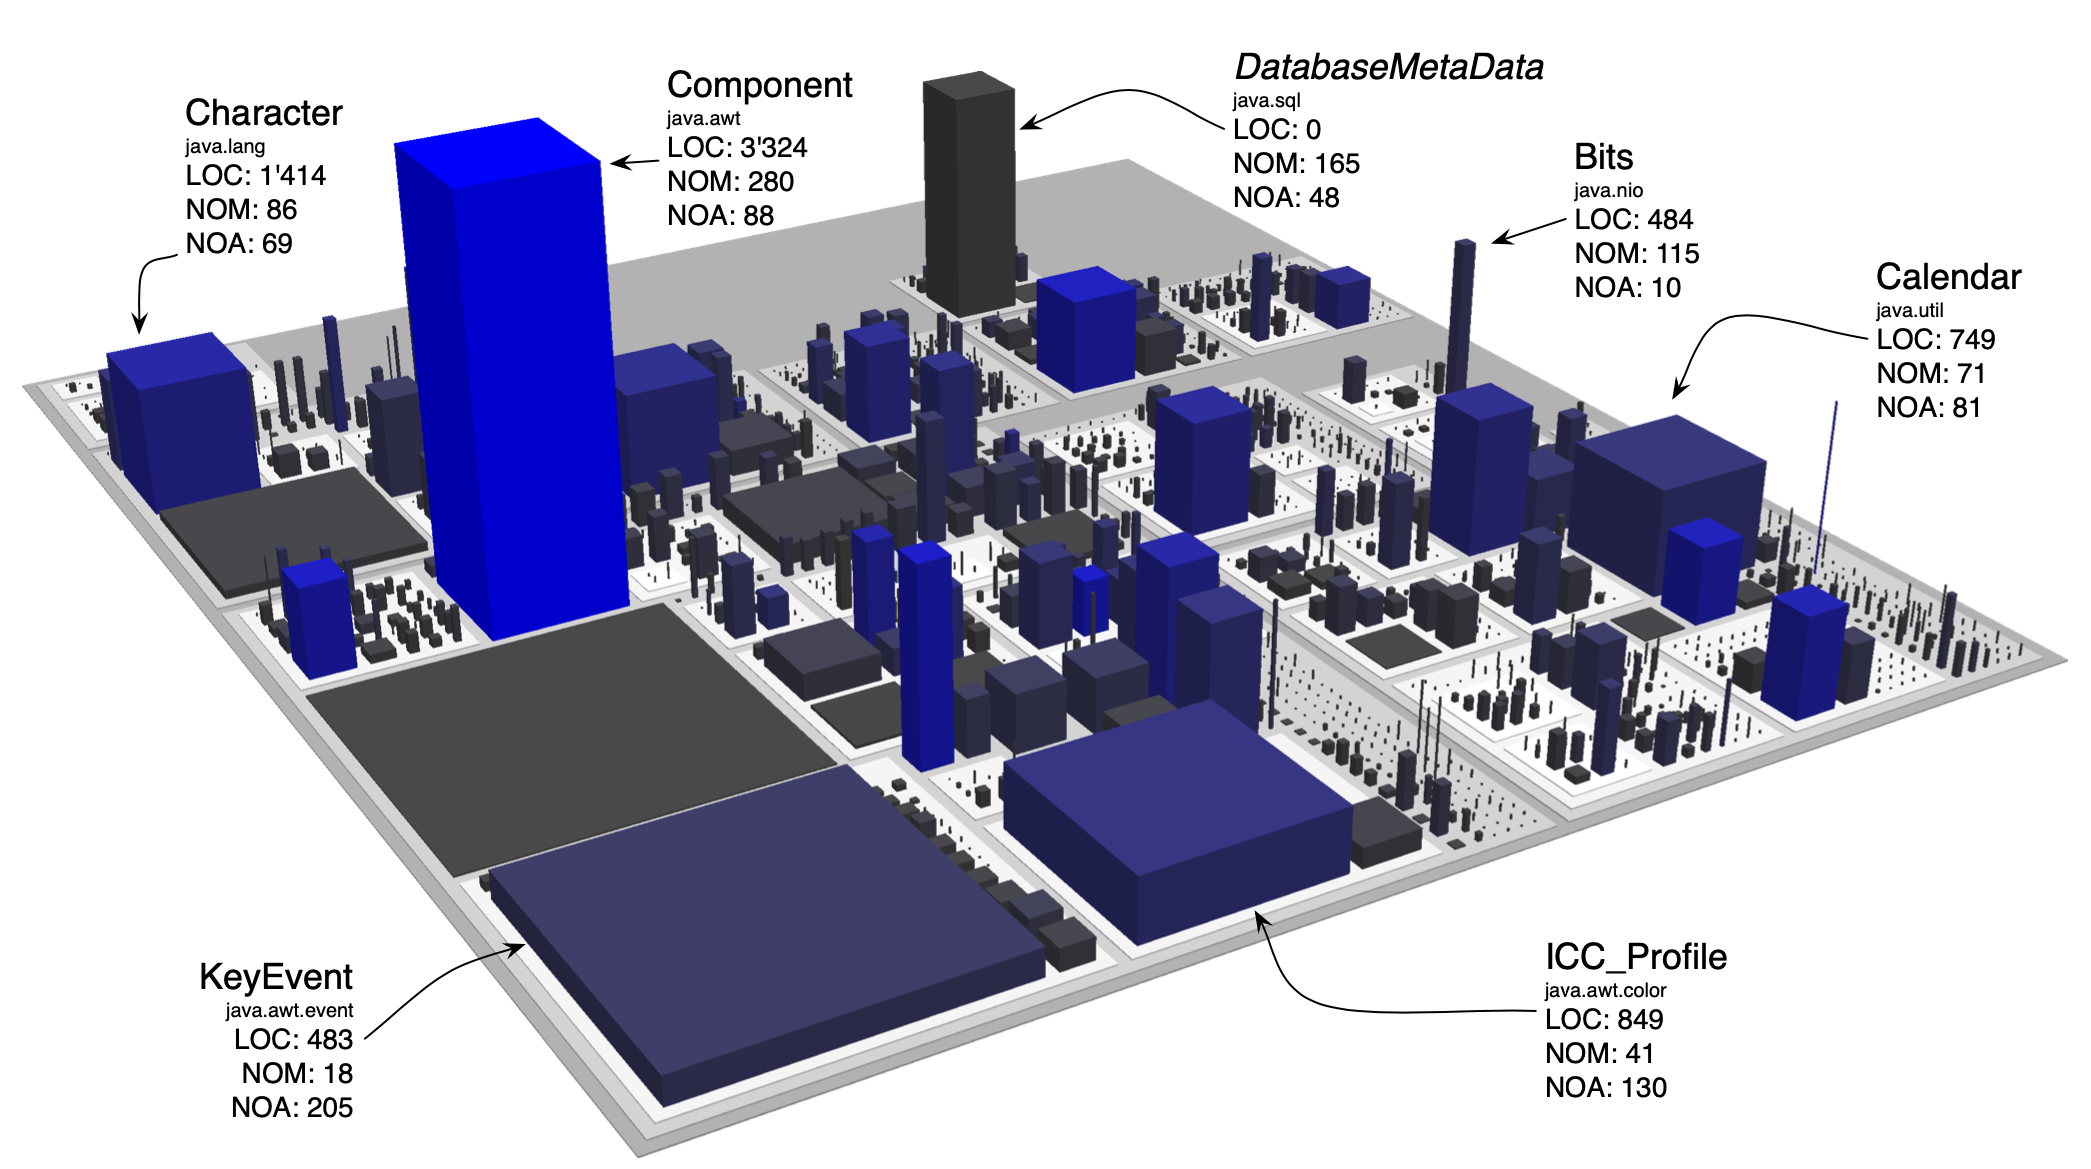
\includegraphics[width=0.9\linewidth]{CodeCity.png} 
  \caption{CodeCity}
\end{figure}

% TODO https://ieeexplore.ieee.org/document/1334769


% ChronoTwigger 2014 https://ieeexplore.ieee.org/abstract/document/6980223
\bigbreak
Ens et al. \cite{Ens2014} applied visual analytics methods to software repositories.
His approach helped users comprehend co-evolution information by visualizing how source and test files were developed together. 
 
% NN 2015 https://ieeexplore.ieee.org/document/7329727
\bigbreak
Kapec et al. \cite{Kapec2015} proposed a graph analysis approach with augmented reality. 
They made a prototype of a tool that provided a graph-based visualization of software, and then they studied some interaction methods to control it with augmented reality.
 
% CuboidMatrix 2016 https://ieeexplore.ieee.org/document/7780168
\bigbreak
Schneider et al. \cite{Schneider2016} presented a tool, CuboidMatrix, that employed a space-time cube metaphor to visualize a software system. 
A space-time cube is a well-known 3D representation of an evolving dynamic graph. 
 
% CityVR 2017 https://ieeexplore.ieee.org/abstract/document/8094470
\bigbreak
Merino et al. \cite{Merino2017} aimed to augment software visualization with gamification. 
They introduced CityVR, a tool that displays a software system through the city metaphor with a 3D environment. 
Working with virtual reality, they scaled the city visualization to the physically available space in the room. 
Therefore, developers needed to walk to navigate the system. 

\begin{figure}[H]
  \minipage{0.32\textwidth}
    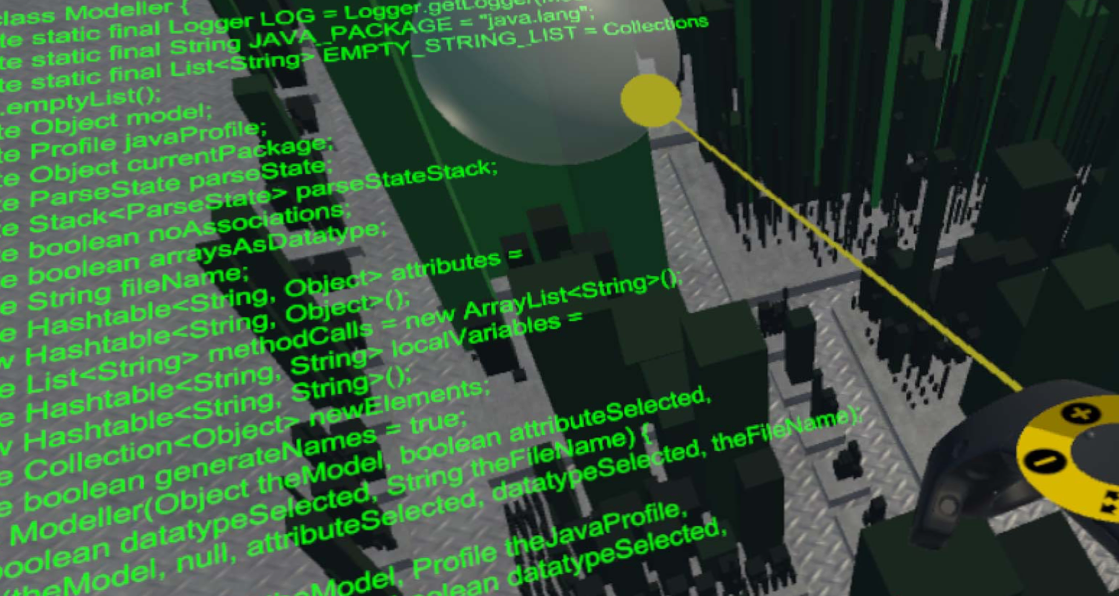
\includegraphics[width=\linewidth]{CityVR.png}
    \caption{CityVR}
  \endminipage\hfill
  \minipage{0.32\textwidth}
    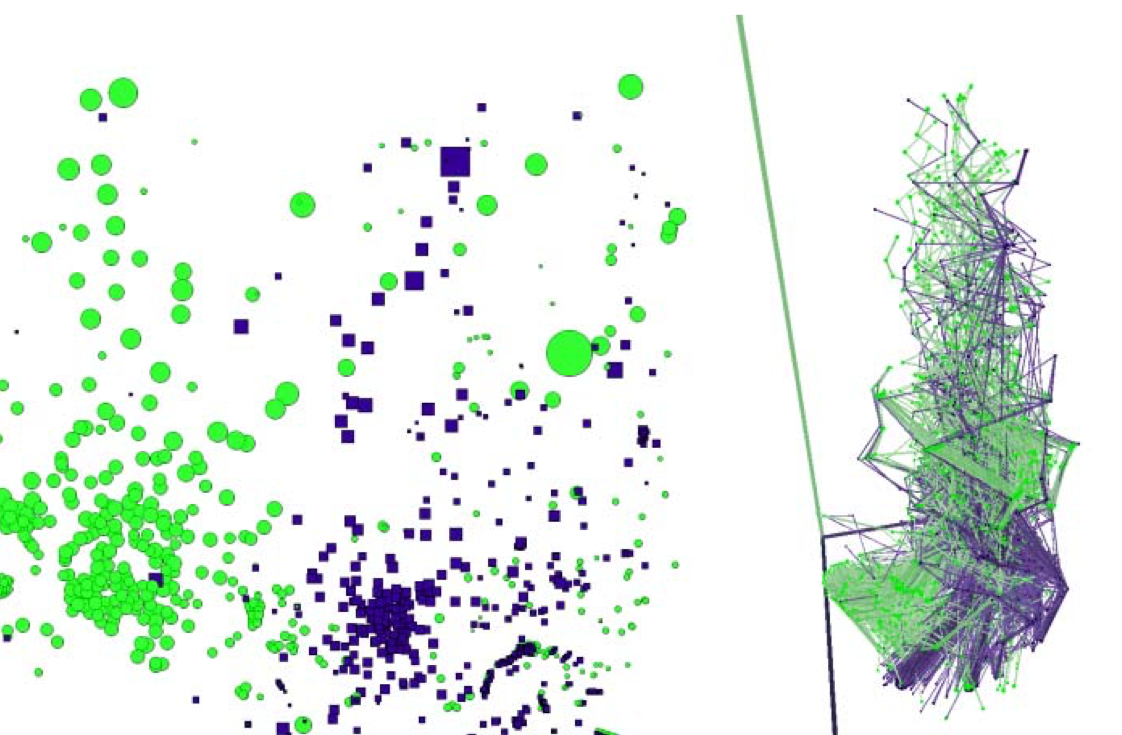
\includegraphics[width=\linewidth]{ChronoTwigger.png}
    \caption{ChronoTwigger}
  \endminipage\hfill
  \minipage{0.32\textwidth}%
    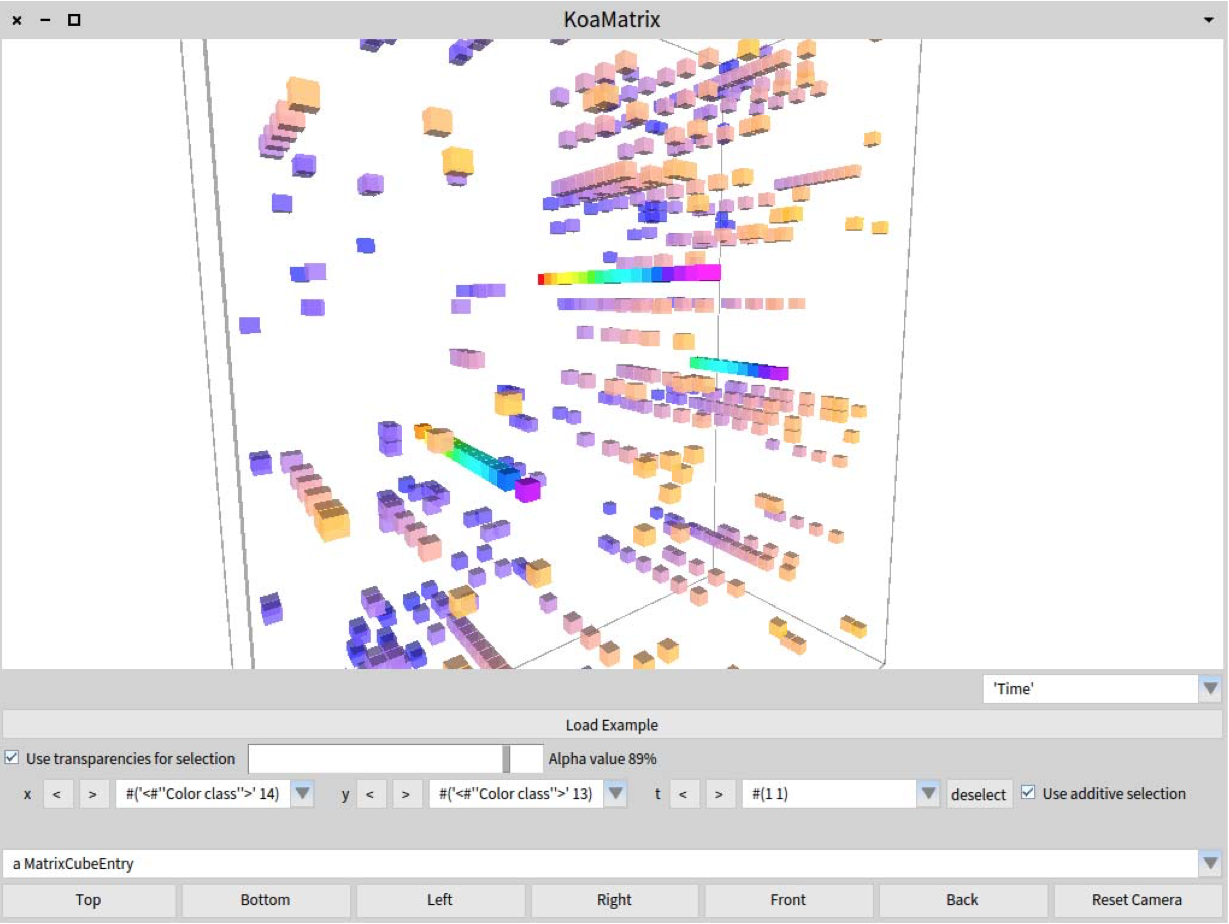
\includegraphics[width=\linewidth]{CuboidMatrix.png}
    \caption{CuboidMatrix}
  \endminipage
  \end{figure}
  


% Code Park 2017 https://ieeexplore.ieee.org/abstract/document/8091185
\bigbreak
Khaloo et al. \cite{Khaloo2017} revised the idea of gamification with a 3D park-like environment. They mapped each class in the codebase with a facility. The wall structure depended on the class's constituent parts, e.g., methods and signatures. 

% Evo-Clocks 2019 https://ieeexplore.ieee.org/document/8900965
\bigbreak
Finally, we mention Alexandru et al., who proposed a method to visualize software structure and evolution, 
with reduced accuracy and a fine-grained highlighting of changes in individual components \cite{Alexandru2019}. 

\begin{figure}[H]
  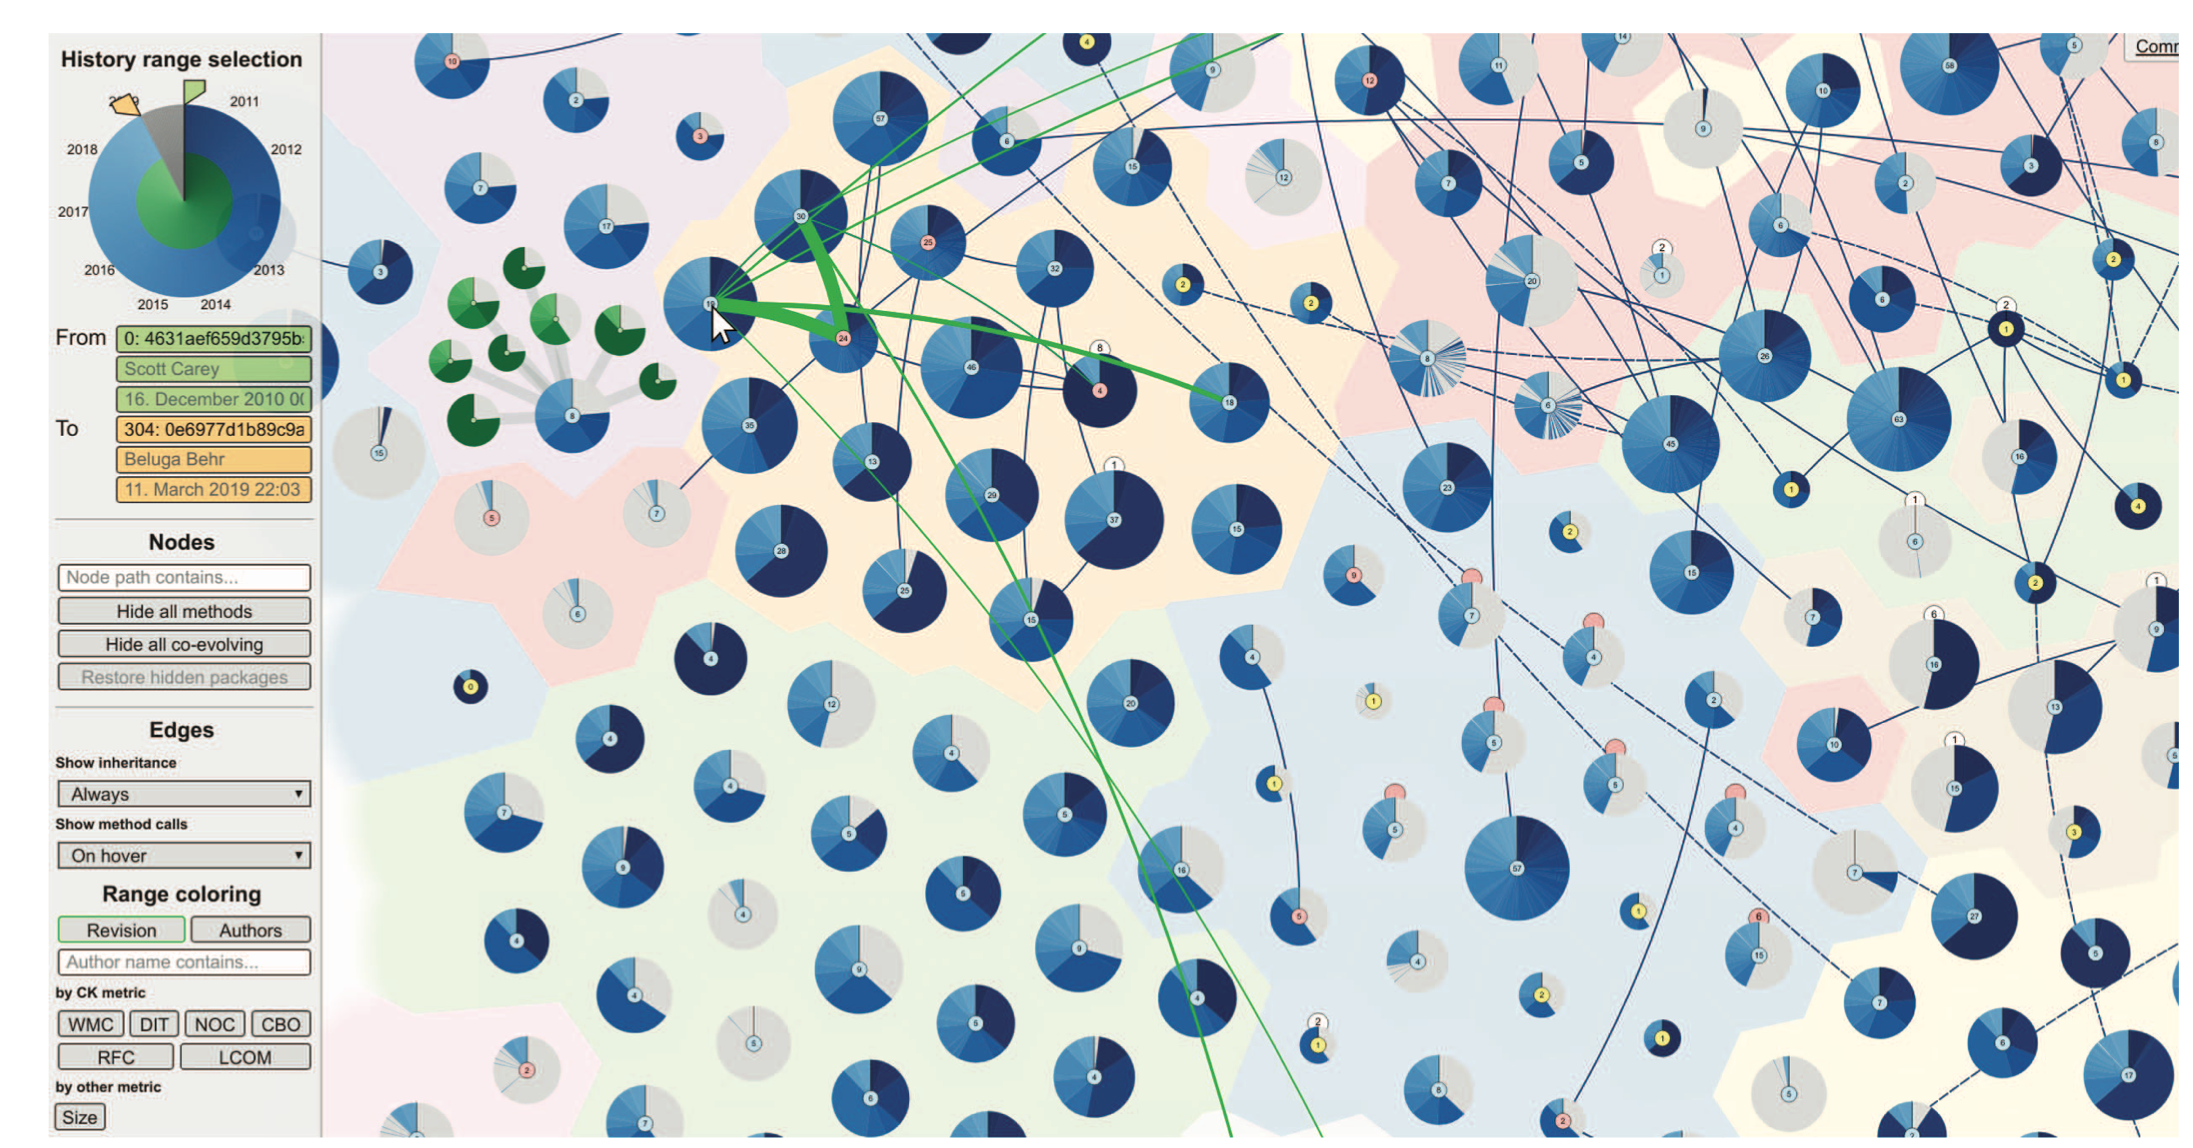
\includegraphics[width=0.9\linewidth]{Alexandru_EvoClock.png} 
  \caption{Evo-Clock}
\end{figure}


\section{Analysis of software evolution}

Software repositories contain historical data about the evolution of a software system. 
Thanks to the spread of the git protocol, and consequently of GitHub, 
Mining Software Repositories (MSR) has become a popular research field. 

\bigbreak
D'Ambros et al. in \cite{SoftwareEvolution} presented several analysis and visualization techniques to understand software evolution. 
They developed an approach based on a Release History Database (RHDB). 
It is a database that stores historical information about source code and bugs. 
The strength of RHDB was the association between historical versions of flies and bugs. 
Having this information stored on a database, they were able to run some evolution analysis to obtain information such as how many developers worked on a file to fix a bug or how the effort was to fix it.  

Finally, they concluded by evidencing two main challenges in MSR:
\begin{itemize}
  \item Technical challenge: repositories contain a sheer amount of data, posing scalability problems. 
  \item Conceptual challenge: how to do something meaningful with the collected data. 
  Most of the approaches present in literature to visualize software evolution have unanswered questions about the effectiveness of the comprehension. 
\end{itemize}

\begin{figure}[H]
  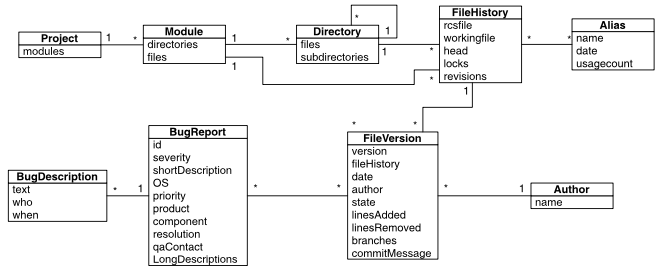
\includegraphics[width=0.9\linewidth]{RHDB.png} 
  \caption{RHDB}
  \label{fig:RHDB}
\end{figure}
 


% The promises and perils of mining GitHub  https://dl.acm.org/doi/abs/10.1145/2597073.2597074
\bigbreak
In 2022, the number of GitHub repositories lays around 200 million.
Even if it seems a promising data source, Kalliamvakou et al. raised some issues with its mining. \cite{Kalliamvakou2014} 
For example, they evidenced that a repository does not always match a project. 
A reason for this can be found in the fact that most repositories had had very few commits before becoming inactive.
Over 70 percent of the GitHub projects were personal when they did their research, and some weren't used for software development. 
Finally, the last perils they raised were related to GitHub features that software developers do not properly use.
They considered only projects with a good balance between the number of commits, 
the number of pull requests, and the number of contributors to find actively developed repositories. 
 

% PyDriller https://dl.acm.org/doi/abs/10.1145/3236024.3264598
\bigbreak
Spadini, Aniche and Bacchelli \cite{Spadini2018}. They developed a Python framework called PyDriller, enabling users to mine software repositories. 
Their tool can be used to extract information about the evolution of a software system from any git repository.  

\bigbreak
We also mention the work done by Salis and Spinellis \cite[]{Salis2019}.
They introduced RepoFS, a tool that allows navigating a git repository as a file system. 
Their approach sees commits, branches, and tags as a separate directory tree. 
Figure \ref{fig:RepoFS} shows an example of a repository data structure. 

\begin{figure}[H]
  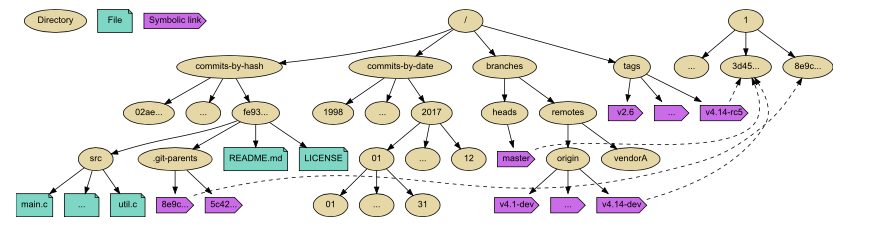
\includegraphics[width=0.9\linewidth]{Salis2019.png} 
  \caption{RepoFS}
  \label{fig:RepoFS}
\end{figure}

\bigbreak
Clem and Thomson \cite[]{Clem2021}, members of the semantic code team at GitHub, built a static analyzer of repositories to implement symbolic code navigation. 
That feature was released on GitHub some years ago and let developers click on a name identifier to navigate to the definition of that entity. 
They were looking for a solution that would not bring them scalability problems. 
Moreover, they built the symbolic navigation feature around some ideas like:
\begin{itemize}
  \item Zero configuration needed by the owner of a repository
  \item Incrementality of the process. There was no need to process the entire repository for every commit made by a developer. Instead, they analyzed only the files that had changed. 
  \item Language agnosticism of the static analysis. 
\end{itemize}

Working on that feature, they recognized the difficulty of scaling a static analysis like that regarding human behavior. 
Nevertheless, their idea was to have an agnostic static analyzer, but they could not reach this goal, and they were forced to implement it for just nine programming languages.  

\section{Data sonification}

External auditory representations of programs (known as "program auralisation") is a research field that 
is getting even more interest in the recent years.

% InfoSound https://ieeexplore.ieee.org/document/205229
\bigbreak
Sonnenwald et al. made one of the first attempts. \cite{Sonnenwald1990}
They tried to enhance the comprehension of complex applications by playing music and special sound effects. 
This approach was supported by a tool called InfoSound
It was mainly adopted to understand the program's behavior. 

\bigbreak
Many other researchers followed this first technique. To cite some of them, DiGiano and Baecker \cite{DiGiano1993} made LogoMedia, a tool to associate non-speech
 audio with program events while the code is being developed. 
Jameson \cite{Jameson1994}] developed Sonnet, audio-enhanced monitoring and debugging tool.  
Alty and Vickers \cite{Vickers2003} had a similar idea. Using a structured musical framework, they could map the execution behavior of a program to locate and diagnose software errors. 
 
% EXTERNAL AUDITORY REPRESENTATIONS OF PROGRAMS https://smartech.gatech.edu/bitstream/handle/1853/50854/Vickers2004a.pdf?sequence=1&
\bigbreak
Despite the usefulness of these tools, they adopted an essential kind of mapping, and thus they had a limited musical representation. 
Vickerts \cite{Vickers2004} evidenced the necessity of a multi-threaded environment to enhance the comprehension given by the musical representation. 
He proposed adopting an orchestral model of families of timbres to enable programmers to distinguish between different activities of different threads.

\bigbreak
The size and the complexity of systems can represent a problem for the effectiveness of a visual representation of a software system.
Having a large number of visual information, observers might find it difficult to focus only on the relevant aspects. 
% CocoViz https://ieeexplore.ieee.org/document/5070558
Boccuzzo and Gall \cite{Boccuzzo2009} supported software visualization with sonification. 
They used audio melodies to improve navigation and comprehension of their tool, called CocoViz.
Their ambient audio software exploration approach exploited audio to describe the position of an entity in the space intuitively. 
Thanks to the adoption of surround sound techniques, the observers perceived the origin of an audio source so it could adjust their navigation in the visualization.
Each kind of entity played a different sound based on mapping criteria.

\begin{figure}[H]
  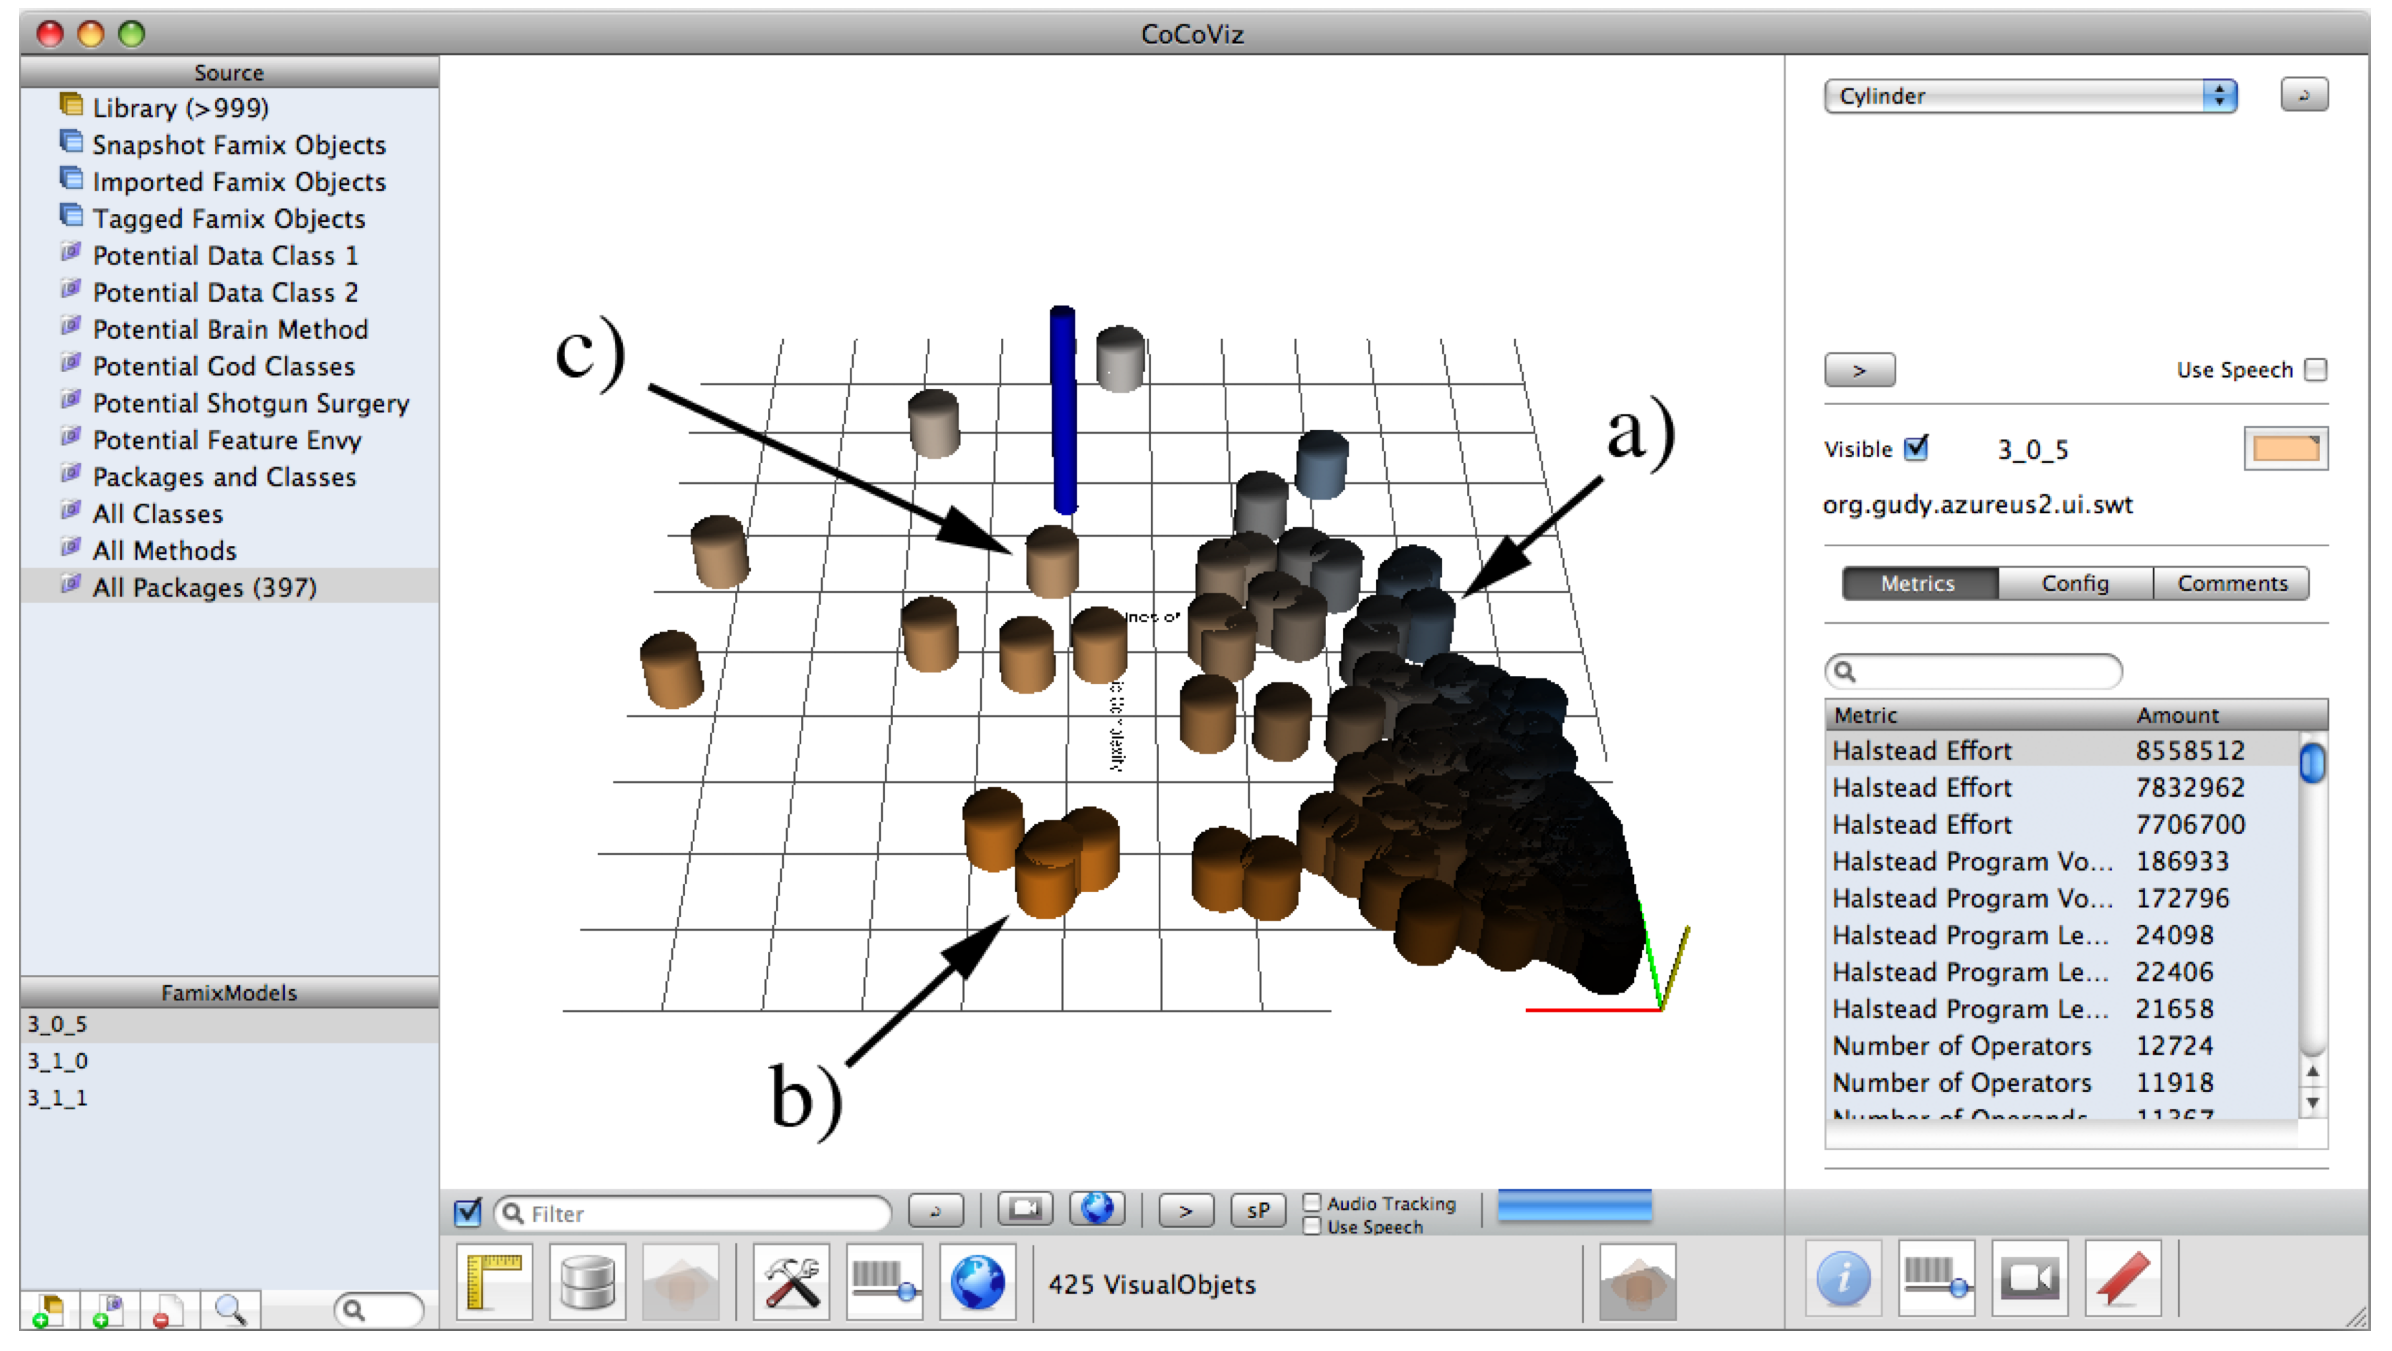
\includegraphics[width=0.9\linewidth]{CocoViz.png} 
  \caption{CocoViz}
\end{figure}


 
% Orchestrating change: An artistic representation of software evolution https://ieeexplore.ieee.org/document/6747192 
\bigbreak
McIntosh et al. \cite{McIntosh2014} explored the use of a parameter-based sonification to produce a musical interpretation of the evolution of a software system.
Their technique mapped musical rests to an inactive period of development and consonance and dissonance to interesting phenomena (like co-changing of components).
% Software Musification https://ieeexplore.ieee.org/document/8107958
\bigbreak
Finally, Mancino and Scanniello \cite{Mancino2017} presented an approach to transforming source code metrics into a musical score that can be both visualized and played. 


\section{Conclusion}

We have seen many different techniques and tools focused on visualizing the source code of software systems, their evolution, or some metrics.
Our approach won't consider the source code visualization. Instead, it is focused on the evolution of a software system and how some metrics run over its history. 
Moreover, in contrast to what some tools did, we are not focused on the evolution code bugs.\\
\\
The codebase of a system is composed of a group of files. In our approach, each file represents a system entity that mutates over time.
It is not based on a previously identified metaphor, such as CodeCity or CityVR with the city metaphor.
We created a new layout where the position of each entity is defined by its discovery time. \\
\\
At present, git has become de-facto the standard tool for version control. 
Having this in mind, we aim to find a suitable model to represent the histories of mined git repositories.
Therefore, we created a model inspired by the EvolutionMatrix, but with some adjustments to make it work with git. \\
\\
As the GitHub team did, we propose a scalable approach that works with large repositories. 
It differs from what they did because we are not focused on a semantic analysis of the source code; instead, we need to extract some metrics. 
Moreover, in contrast to what they did, our technique is purely language-agnostic.\\
\\
Finally, we augmented the effectiveness of our approach with an external auditory representation. 
Conversely to what they did in the first approaches, we used a multithreaded environment to play the musical notes. 
Whereas CocoViz used audio melodies to support the navigation of space created for the visualization, we mapped sounds to the magnitudes of changes in a given moment. 





